% !TeX program = lualatex
% ================================================================
% Polish Parallel Text Version of AccountsWorksheetAuxillarySlides
%
% Generated by the server using the following settings:
%
%   language            Polish (pol)
%   text direction      left to right
%   font                Noto Serif
%   fallback font       Noto Serif
%   built from          latex/worksheets/percentages/savingsInvestigationTask/accountsWorksheetAuxillarySlides.tex
%   vocabulary key      latex/worksheets/percentages/savingsInvestigationTask/accountsWorksheetAuxillarySlides/L2/pol/accountsWorksheetAuxillarySlides_polishKey.tex
%   tier 3 vocabulary   green   RGB 0 128 0
%   English text        black   RGB 0 0 0
%   Polish text         purple  RGB 112 48 160
%   layout macros       version 3
%
% Please don't edit any information in this comment block - the server
% compares it against the current settings and rebuilds this file when
% they differ, so changes here would be overwritten. However, feel free
% to make updates to the LaTeX below if you want to edit it.
% ================================================================

\documentclass[aspectratio=169,12pt]{beamer}
% ================================================================
% Copied from the English sheet this was translated from, so that
% anything it sets up for itself still works here
% ================================================================
\usetheme{default}
\setbeamertemplate{navigation symbols}{}

\usepackage[T1]{fontenc}
% lining, tabular figures: digits sit on the baseline and money columns line up
\usepackage[sfdefault,scaled=0.92,lining,tabular]{FiraSans}
\usepackage{tikz}
\usetikzlibrary{overlay-beamer-styles}
\usepackage{pgfplots}
\pgfplotsset{compat=1.18}
\usepackage{booktabs}
\usepackage{array}
\usepackage{colortbl}
\usepackage{tcolorbox}
\tcbuselibrary{skins}
% Maths is set in the text font, so the formulas and the prose match.
\usepackage[italic]{mathastext}

% ---------------- bank colours (match the worksheets) -------------
\definecolor{metroline}{HTML}{1F4E9C}
\definecolor{virgo}{HTML}{C62828}
\definecolor{coventree}{HTML}{2E7D32}
\definecolor{starlight}{HTML}{6A1B9A}
\definecolor{chace}{HTML}{00796B}
\definecolor{tesbury}{HTML}{E65100}
\definecolor{santandra}{HTML}{C62828}
\definecolor{nationworth}{HTML}{AD1457}
\definecolor{halifield}{HTML}{00796B}
\definecolor{answer}{HTML}{B3005E}

% ---------------- neutral palette ---------------------------------
\definecolor{slidehead}{HTML}{1C2B3A}   % titles and headings
\definecolor{ink}{HTML}{212B36}         % body text
\definecolor{inkmuted}{HTML}{6B7A8A}    % labels, axes, captions
\definecolor{hairline}{HTML}{DCE3EA}    % rules and card edges

\setbeamercolor{normal text}{fg=ink}
\setbeamercolor{structure}{fg=slidehead}
\setbeamertemplate{itemize items}[circle]
\arrayrulecolor{hairline}
\setlength{\heavyrulewidth}{0.5pt}
\setlength{\lightrulewidth}{0.4pt}
\renewcommand{\arraystretch}{1.05}

% A quiet frame number in the bottom corner. This counts frames rather
% than slides, so it does not move while a slide is building up.
\setbeamertemplate{footline}{%
  \hfill\textcolor{inkmuted}{\scriptsize\insertframenumber}\hspace*{4mm}%
  \vspace*{1.5mm}}

% ---------------- frame title -------------------------------------
\setbeamercolor{frametitle}{fg=white,bg=slidehead}
\setbeamertemplate{frametitle}{%
  \vskip1mm%
  \begin{tcolorbox}[enhanced,nobeforeafter,width=\linewidth,
      colback=slidehead,colframe=slidehead,arc=3mm,boxrule=0pt,
      left=3.5mm,right=3.5mm,top=1.2mm,bottom=1.2mm]
    \color{white}\large\bfseries\insertframetitle
  \end{tcolorbox}%
  \vskip1mm%
}

% ---------------- rounded cards -----------------------------------
% Flat fill, no outline, and a coloured edge down the left-hand side.
% A card for a table or a piece of explanation.
\newtcolorbox{card}[1][slidehead]{enhanced,nobeforeafter,box align=top,
  colback=#1!6,colframe=#1!6,boxrule=0pt,arc=2.5mm,
  borderline west={2.2pt}{0pt}{#1!75},
  left=3mm,right=3mm,top=1.5mm,bottom=1.5mm,
  halign upper=flush left,
  before upper={\def\cardaccent{#1}}}

% A card for a graph, so the plot sits on white.
\newtcolorbox{plotcard}[1][slidehead]{enhanced,nobeforeafter,box align=top,
  colback=white,colframe=hairline,boxrule=0.5pt,arc=2.5mm,
  left=1mm,right=1mm,top=1mm,bottom=0.5mm}

% A card for the calculation done straight from the formula.
\newtcolorbox{formulacard}[1][slidehead]{enhanced,nobeforeafter,box align=top,
  colback=white,colframe=hairline,boxrule=0.5pt,arc=2.5mm,
  borderline west={2.2pt}{0pt}{#1!75},
  left=3mm,right=3mm,top=1.2mm,bottom=1.2mm,
  fontupper=\footnotesize, halign upper=flush left,
  before upper={\def\cardaccent{#1}}}

% The heading on a card, in the colour of that account.
\newcommand{\cardhead}[1]{{\color{\cardaccent}\bfseries #1}}

% ---------------- answers -----------------------------------------
% \ablank draws an empty answer box on a question slide and \ashow
% prints the answer on the solution slide that follows it. Both take
% the answer as their argument, so the question text can be written
% once and used on both slides.
\newcommand{\ablank}[1]{%
  \tikz[baseline=-0.7ex]{%
    \node[draw=hairline,line width=0.8pt,fill=slidehead!4,
          rounded corners=2pt,minimum width=24mm,minimum height=6mm,
          inner sep=0pt] {};}}
\newcommand{\ashow}[1]{\textcolor{answer}{\textbf{#1}}}

% \pounds usable inside maths
\newcommand{\pnd}{\mbox{\pounds}}

% ---------------- mini-whiteboard and solution banners ------------
\newcommand{\wb}{%
  \tcbox[on line,boxsep=0.8pt,left=4pt,right=4pt,top=1.2pt,bottom=1.2pt,
         colback=white,colframe=white,arc=3.5pt,boxrule=0pt]
        {\color{slidehead}\scriptsize\bfseries MINI-WHITEBOARDS}}

\newcommand{\sol}{%
  \tcbox[on line,boxsep=0.8pt,left=4pt,right=4pt,top=1.2pt,bottom=1.2pt,
         colback=answer,colframe=answer,arc=3.5pt,boxrule=0pt]
        {\color{white}\scriptsize\bfseries SOLUTION}}

% The gap between questions. A question slide has nothing else on it, so
% it can afford to be roomy; the solution slide also carries the working.
\newlength{\qgap}
\setlength{\qgap}{2.5mm}

% The centred block a question slide is set in.
\newenvironment{questionblock}
  {\vspace{2mm}\begin{center}\begin{minipage}{0.72\textwidth}%
   \large\setlength{\qgap}{4mm}}
  {\end{minipage}\end{center}}

% ---------------- a bank name badge ------------------------------
\newcommand{\bank}[2]{%
  \tcbox[on line,boxsep=1pt,left=5pt,right=5pt,top=1.8pt,bottom=1.8pt,
         colback=#1,colframe=#1,arc=4.5pt,boxrule=0pt]
        {\color{white}\small\bfseries #2}}

% ---------------- shared plot style ------------------------------
% Thin grey axes with no arrow tips, faint grid, and a legend that
% floats on the plot rather than sitting in a box.
\pgfplotsset{
  moneyaxis/.style={
    width=6.4cm, height=4.0cm,
    xlabel={years}, ylabel={amount (\pounds)},
    xlabel style={font=\scriptsize,color=inkmuted},
    ylabel style={font=\scriptsize,color=inkmuted},
    tick label style={font=\scriptsize,color=inkmuted},
    grid=major, grid style={hairline,line width=0.4pt},
    axis lines=left,
    axis line style={draw=hairline,line width=0.6pt,-},
    tick style={draw=hairline},
    enlarge x limits=0.06,
    scaled y ticks=false,
    y tick label style={/pgf/number format/fixed,
                        /pgf/number format/1000 sep={}},
    legend style={font=\scriptsize,draw=none,fill=white,
                  fill opacity=0.85,text opacity=1,
                  at={(0.02,0.99)},anchor=north west,
                  inner sep=1.5pt,nodes={inner sep=1.5pt}},
    legend cell align=left,
  }
}

% ---------------- building a table up row by row ------------------
% Each cell is uncovered from overlay #1 onwards. The whole table is
% typeset from the start, so the column widths and the rows below it
% do not move as the rows appear.
\newcommand{\rowtwo}[3]{\uncover<#1->{#2} & \uncover<#1->{#3}\\}
\newcommand{\rowthree}[4]{%
  \uncover<#1->{#2} & \uncover<#1->{#3} & \uncover<#1->{#4}\\}

% ---------------- building a graph up point by point --------------
% \pt draws a single point, \seg one straight segment from #3 to #4,
% and \curveseg the piece of a curve between x = #3 and x = #4. Each
% is hidden until overlay #1 rather than left out, so the axis keeps
% its size and the earlier parts of the line stay put.
%   #1 first overlay   #2 plot style   #3, #4 coordinates
\newcommand{\pt}[3]{%
  \addplot[#2,visible on=<#1->,forget plot] coordinates {#3};}
\newcommand{\seg}[4]{%
  \addplot[#2,visible on=<#1->,forget plot] coordinates {#3#4};}
%   #1 first overlay  #2 style  #3 from  #4 to  #5 expression in x
\newcommand{\curveseg}[5]{%
  \addplot[#2,visible on=<#1->,forget plot,domain=#3:#4,samples=41] {#5};}

% Legends are built from \addlegendimage so that they are complete from
% the first overlay, while the plots themselves are all "forget plot".
\newcommand{\legendfor}[2]{\addlegendimage{#1}\addlegendentry{#2}}

% A rounded label marking the years a saver cannot withdraw the money.
%   #1 colour   #2 x position   #3 y position
\newcommand{\lockedlabel}[3]{%
  \node[fill=#1!12,rounded corners=3pt,inner xsep=4pt,inner ysep=2.5pt,
        font=\tiny,text=#1,align=center] at (axis cs:#2,#3) {locked in};}

\title{Savings accounts: which is the best deal?}
\subtitle{Worked examples}
\date{}

% Characters this language's font has not got are borrowed from another,
% rather than being silently dropped - see docs/translated-sheet-latex.md
\directlua{%
  if luaotfload and luaotfload.add_fallback then
    luaotfload.add_fallback("eallatinfallback",
      { "Noto Serif:mode=harf;" })
  else
    tex.error("this luaotfload is too old to register a fallback font")
  end
}
\usepackage[english]{babel}
\babelprovide[import]{polish}
\babelfont[polish]{rm}[Renderer=Harfbuzz, BoldFont={Noto Serif}, ItalicFont={Noto Serif}, BoldItalicFont={Noto Serif}, RawFeature={fallback=eallatinfallback}]{Noto Serif}
\babelfont[polish]{sf}[Renderer=Harfbuzz, BoldFont={Noto Serif}, ItalicFont={Noto Serif}, BoldItalicFont={Noto Serif}, RawFeature={fallback=eallatinfallback}]{Noto Serif}
\newcommand{\ealtext}[1]{\foreignlanguage{polish}{#1}}
\newcommand{\ealtextblock}[1]{{\raggedright\foreignlanguage{polish}{#1}\par}}
% ================================================================
% EAL layout helpers
% ================================================================
\usepackage{xcolor}

\definecolor{ealkeycolour}{RGB}{0,128,0}
\definecolor{ealenglish}{RGB}{0,0,0}
\definecolor{ealtwocolour}{RGB}{112,48,160}

\newsavebox{\ealboxen}
\newsavebox{\ealboxtr}
\newlength{\ealglosswd}
\newlength{\ealglossraise}
\setlength{\ealglossraise}{1.15em}

% a tier 3 word, in English and in translation alike
\newcommand{\ealkey}[1]{\textcolor{ealkeycolour}{#1}}
\newcommand{\ealkeytr}[1]{\textcolor{ealkeycolour}{\ealtext{#1}}}

% One translated word above one English word. Built from kernel
% primitives, never a tabular, which would break wherever the sheet
% loads array, booktabs or tabularx. The box is as wide as the wider of
% the two, so a long translation pushes its neighbours aside instead of
% overlapping them, and it claims its full height so a table row or a
% TikZ node makes room for it.
\newcommand{\ealgloss}[2]{%
  \sbox{\ealboxen}{\ealkey{#1}}%
  \sbox{\ealboxtr}{\small\textcolor{ealtwocolour}{\ealtext{#2}}}%
  \setlength{\ealglosswd}{\wd\ealboxen}%
  \ifdim\wd\ealboxtr>\ealglosswd\setlength{\ealglosswd}{\wd\ealboxtr}\fi
  \leavevmode
  \makebox[\ealglosswd][c]{%
    \makebox[0pt][c]{\usebox{\ealboxen}}%
    \makebox[0pt][c]{\raisebox{\ealglossraise}{\usebox{\ealboxtr}}}%
  }%
}

% opens up line spacing around a block of glosses, so the raised
% translations sit clear of the line above
\newenvironment{ealglossed}{\par\linespread{2.1}\selectfont\ignorespaces}{\par}

% a whole translated sentence above its English counterpart. block level,
% so it does not belong inside a tabular cell
\newcommand{\ealpara}[2]{%
  \par\addvspace{0.5\baselineskip}%
  {\color{ealtwocolour}\ealtextblock{#1}}%
  \penalty200
  {\color{ealenglish}#2\par}%
  \addvspace{0.5\baselineskip}%
}

\begin{document}

\begin{frame}[plain]
  \vfill
  \hspace*{6mm}%
  \begin{minipage}{0.86\textwidth}
    {\small\bfseries \ealpara{PRZYKŁADY ROZWIĄZANE}{WORKED EXAMPLES}}
    \vspace{3mm}
    {\fontsize{24}{28}\selectfont\bfseries
     \ealpara{Konta oszczędnościowe: która oferta jest najlepsza?}{Savings accounts:\\which is the best deal?}}
    \vspace{4mm}
    \textcolor{slidehead!75}{\rule{28mm}{2.2pt}}
    \vspace{4mm}
    {\small \ealpara{Wszystkie nazwy banków i \ealkeytr{wielkości ilorazowe} \ealkeytr{odsetek} są wymyślone.}{All bank names and \ealkey{interest} \ealkey{rates} are made up.}}
  \end{minipage}
  \vfill
\end{frame}

% =================================================================
\begin{frame}{Two ways of paying \ealkey{interest}}
\ealpara{Dwa sposoby płacenia \ealkeytr{odsetek}}{Two ways of paying \ealkey{interest}}
\begin{columns}[T,onlytextwidth]
\begin{column}{0.48\textwidth}
  \begin{card}[coventree]
    \ealpara{\ealkeytr{Procent prosty}}{\textbf{\ealkey{Simple interest}}}
    \vspace{1mm}
    \footnotesize
    \ealpara{\ealkeytr{Odsetki} są obliczane od kwoty, którą najpierw wpłaciłeś, co roku.}{\ealkey{Interest} is worked out on the amount you first paid in, every year.}
    \vspace{1.5mm}

    \ealpara{\pounds200 przy 10\% \ealkeytr{procencie prostym}:}{\pounds200 at 10\% \ealkey{simple interest}:}
    \vspace{1mm}
    \begin{tabular}{@{}lll@{}}
      \rowthree{2}{Year 1}{\pounds20}{\pounds220}
      \rowthree{3}{Year 2}{\pounds20}{\pounds240}
      \rowthree{4}{Year 3}{\pounds20}{\pounds260}
    \end{tabular}\\[1.5mm]
    \uncover<5->{\ealpara{\ealkeytr{Odsetki} wynoszą \pounds20 co roku.}{The \ealkey{interest} is \pounds20 every year.}}
  \end{card}
\end{column}
\begin{column}{0.48\textwidth}
  \begin{card}[starlight]
    \ealpara{\ealkeytr{Procent składany}}{\textbf{\ealkey{Compound interest}}}
    \vspace{1mm}
    \footnotesize
    \ealpara{\ealkeytr{Odsetki} są obliczane od kwoty na koncie, więc zarabiamy \ealkeytr{odsetki} od \ealkeytr{odsetek}.}{\ealkey{Interest} is worked out on the amount in the account, so we earn \ealkey{interest} on our \ealkey{interest}.}
    \vspace{1.5mm}

    \ealpara{\pounds200 przy 10\% \ealkeytr{procencie składanym}:}{\pounds200 at 10\% \ealkey{compound interest}:}
    \vspace{1mm}
    \begin{tabular}{@{}lll@{}}
      \rowthree{2}{Year 1}{\pounds20.00}{\pounds220.00}
      \rowthree{3}{Year 2}{\pounds22.00}{\pounds242.00}
      \rowthree{4}{Year 3}{\pounds24.20}{\pounds266.20}
    \end{tabular}\\[1.5mm]
    \uncover<5->{\ealpara{\ealkeytr{Odsetki} rosną co roku.}{The \ealkey{interest} grows each year.}}
  \end{card}
\end{column}
\end{columns}

\vspace{2mm}
\uncover<5->{%
\begin{formulacard}[slidehead]
  \ealpara{Te dwa \ealkeytr{wzory}.}{The two \ealkey{formulas}.}
  \ealpara{$P$ to kwota wpłacona, $r$ to \ealkeytr{wielkość ilorazowa} \ealkeytr{odsetek} zapisana jako \ealkeytr{ułamek dziesiętny}, a $n$ to liczba lat.}{$P$ is the amount paid in, $r$ is the \ealkey{interest} \ealkey{rate} written as a \ealkey{decimal} and $n$ is the number of years.}
  \vspace{1mm}
  \centering
  \ealpara{\ealkeytr{procent prosty}: \ealkeytr{suma} $= P(1+rn)$ \qquad \ealkeytr{procent składany}: \ealkeytr{suma} $= P(1+r)^{n}$}{\ealkey{simple interest}: \ealkey{total} $= P(1+rn)$ \qquad\qquad \ealkey{compound interest}: \ealkey{total} $= P(1+r)^{n}$}
\end{formulacard}}
\end{frame}

% =================================================================
\begin{frame}{\bank{coventree}{Coventree} Standard Saver: 5\% \ealkey{simple interest}}
\ealpara{\bank{coventree}{Coventree} Standard Saver: 5\% \ealkeytr{procent prosty}}{\bank{coventree}{Coventree} Standard Saver: 5\% \ealkey{simple interest}}
\ealpara{Fay wpłaca \pounds250 i zostawia je na 3 lata.}{\textbf{Fay puts in \pounds250 and leaves it for 3 years.}}
\vspace{0.6mm}

\begin{columns}[T,onlytextwidth]
\begin{column}{0.44\textwidth}
  \begin{card}[coventree]
    \footnotesize
    \ealpara{5\% z \pounds250 to \pounds12.50, a konto wypłaca to \emph{co rok}.}{5\% of \pounds250 is \pounds12.50, and the account pays that \emph{every} year.}
    \vspace{1.5mm}
    \begin{tabular}{@{}lrr@{}}
      \toprule
      & \ealkey{interest} & \ealkey{total}\\
      \midrule
      \rowthree{1}{Start}{}{\pounds250.00}
      \rowthree{2}{Year 1}{\pounds12.50}{\pounds262.50}
      \rowthree{3}{Year 2}{\pounds12.50}{\pounds275.00}
      \rowthree{4}{Year 3}{\pounds12.50}{\pounds287.50}
      \bottomrule
    \end{tabular}
  \end{card}

  \vspace{1.2mm}
  \uncover<5->{%
  \begin{formulacard}[coventree]
    \ealpara{Stosując \ealkeytr{wzór}}{Using the \ealkey{formula}}
    \vspace{0.6mm}
    \ealpara{\ealkeytr{odsetki} $= P \times r \times n$}{\ealkey{interest} $= P \times r \times n$}
    \vspace{0.4mm}
    \hspace*{3mm}$= \pnd 250 \times 0.05 \times 3 = \pnd 37.50$
    \vspace{0.4mm}
    \ealpara{\ealkeytr{suma} $= \pnd 250 + \pnd 37.50 = \pnd 287.50$}{\ealkey{total} $= \pnd 250 + \pnd 37.50 = \pnd 287.50$}
  \end{formulacard}}
\end{column}
\begin{column}{0.54\textwidth}
  \begin{plotcard}[coventree]
  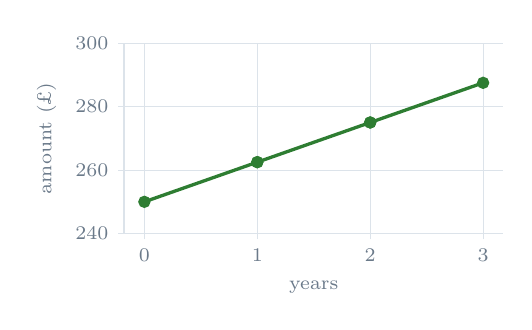
\begin{tikzpicture}
    \begin{axis}[moneyaxis, xmin=0,xmax=3,ymin=240,ymax=300,xtick={0,1,2,3}]
      \pt{1}{coventree,mark=*,mark size=1.6pt}{(0,250)}
      \seg{2}{coventree,very thick,mark=*,mark size=1.6pt}{(0,250)}{(1,262.5)}
      \seg{3}{coventree,very thick,mark=*,mark size=1.6pt}{(1,262.5)}{(2,275)}
      \seg{4}{coventree,very thick,mark=*,mark size=1.6pt}{(2,275)}{(3,287.5)}
    \end{axis}
  \end{tikzpicture}
  \end{plotcard}\\[1mm]
  \uncover<5->{\footnotesize\ealpara{\ealkeytr{Procent prosty} daje \textbf{linię prostą}.}{\ealkey{Simple interest} gives a \textbf{straight line}.}}
\end{column}
\end{columns}
\end{frame}

% =================================================================
\newcommand{\amaraQuestions}[1]{%
  \ealpara{Ile \ealkeytr{odsetek} każdego roku?}{How much \ealkey{interest} each year? \hfill #1{\pounds12}}\vspace{\qgap}
  \ealpara{Ile \ealkeytr{odsetek} łącznie?}{How much \ealkey{interest} altogether? \hfill #1{\pounds48}}\vspace{\qgap}
  \ealpara{\ealkeytr{Suma} na końcu?}{\ealkey{Total} at the end? \hfill #1{\pounds168}}}

\begin{frame}{\wb\ \ \bank{metroline}{Metroline Bank} 10\% \ealkey{simple interest}}
\ealpara{\wb\ \ \bank{metroline}{Metroline Bank} 10\% \ealkeytr{procent prosty}}{\wb\ \ \bank{metroline}{Metroline Bank} 10\% \ealkey{simple interest}}
\begin{questionblock}
  \ealpara{Amara wpłaca \pounds120 i zostawia je na 4 lata.}{\textbf{Amara puts in \pounds120 and leaves it for 4 years.}}
  \vspace{7mm}
  \amaraQuestions{\ablank}
\end{questionblock}
\end{frame}

\begin{frame}{\sol\ \ \bank{metroline}{Metroline Bank} 10\% \ealkey{simple interest}}
\ealpara{\sol\ \ \bank{metroline}{Metroline Bank} 10\% \ealkeytr{procent prosty}}{\sol\ \ \bank{metroline}{Metroline Bank} 10\% \ealkey{simple interest}}
\ealpara{Amara wpłaca \pounds120 i zostawia je na 4 lata.}{\textbf{Amara puts in \pounds120 and leaves it for 4 years.}}
\vspace{2mm}

\begin{columns}[T,onlytextwidth]
\begin{column}{0.5\textwidth}
  \amaraQuestions{\ashow}

  \vspace{4mm}
  \uncover<6->{%
  \begin{formulacard}[metroline]
    \ealpara{Stosując \ealkeytr{wzór}}{Using the \ealkey{formula}}
    \vspace{0.6mm}
    \ealpara{\ealkeytr{odsetki} $= P \times r \times n$}{\ealkey{interest} $= P \times r \times n$}
    \vspace{0.4mm}
    \hspace*{3mm}$= \pnd 120 \times 0.10 \times 4 = \pnd 48$
    \vspace{0.4mm}
    \ealpara{\ealkeytr{suma} $= \pnd 120 + \pnd 48 = \pnd 168$}{\ealkey{total} $= \pnd 120 + \pnd 48 = \pnd 168$}
  \end{formulacard}}
\end{column}
\begin{column}{0.46\textwidth}
  \begin{card}[metroline]
    \footnotesize
    \begin{tabular}{@{}lrr@{}}
      \toprule
      & \ealkey{interest} & \ealkey{total}\\
      \midrule
      \rowthree{1}{Start}{}{\pounds120}
      \rowthree{2}{Year 1}{\pounds12}{\pounds132}
      \rowthree{3}{Year 2}{\pounds12}{\pounds144}
      \rowthree{4}{Year 3}{\pounds12}{\pounds156}
      \rowthree{5}{Year 4}{\pounds12}{\pounds168}
      \bottomrule
    \end{tabular}
  \end{card}
\end{column}
\end{columns}
\end{frame}

% =================================================================
\begin{frame}{\bank{starlight}{Starlight Bank} Steady Saver: 5\% \ealkey{compound interest}}
\ealpara{\bank{starlight}{Starlight Bank} Steady Saver: 5\% \ealkeytr{procent składany}}{\bank{starlight}{Starlight Bank} Steady Saver: 5\% \ealkey{compound interest}}
\ealpara{Fay wpłaca \pounds250 i zostawia je na 3 lata.}{\textbf{Fay puts in \pounds250 and leaves it for 3 years.}}
\vspace{1mm}

\begin{columns}[T,onlytextwidth]
\begin{column}{0.44\textwidth}
  \begin{card}[starlight]
    \footnotesize
    \ealpara{Mnożymy przez $1.05$ co roku.}{We multiply by $1.05$ each year.}
    \vspace{1.5mm}
    \begin{tabular}{@{}lrr@{}}
      \toprule
      & \ealkey{interest} & \ealkey{total}\\
      \midrule
      \rowthree{1}{Start}{}{\pounds250.00}
      \rowthree{2}{Year 1}{\pounds12.50}{\pounds262.50}
      \rowthree{3}{Year 2}{\pounds13.13}{\pounds275.63}
      \rowthree{4}{Year 3}{\pounds13.78}{\pounds289.41}
      \bottomrule
    \end{tabular}
  \end{card}

  \vspace{0.8mm}
  \uncover<5->{%
  \begin{formulacard}[starlight]
    \ealpara{Stosując \ealkeytr{wzór}}{Using the \ealkey{formula}}
    \vspace{0.6mm}
    \ealpara{\ealkeytr{suma} $= P(1+r)^{n}$}{\ealkey{total} $= P(1+r)^{n}$}
    \vspace{0.4mm}
    \hspace*{3mm}$= \pnd 250 \times 1.05^{3} = \pnd 289.41$
    \vspace{0.4mm}
    \ealpara{\ealkeytr{odsetki} $= \pnd 289.41 - \pnd 250 = \pnd 39.41$}{\ealkey{interest} $= \pnd 289.41 - \pnd 250 = \pnd 39.41$}
  \end{formulacard}}
\end{column}
\begin{column}{0.54\textwidth}
  \begin{plotcard}[starlight]
  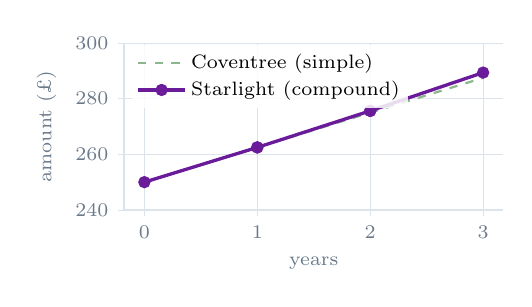
\begin{tikzpicture}
    \begin{axis}[moneyaxis, height=3.7cm,
                 xmin=0,xmax=3,ymin=240,ymax=300,xtick={0,1,2,3}]
      \legendfor{coventree!55,thick,dashed}{Coventree (simple)}
      \legendfor{starlight,very thick,mark=*,mark size=1.6pt}{Starlight (compound)}
      \seg{2}{coventree!55,thick,dashed}{(0,250)}{(1,262.5)}
      \seg{3}{coventree!55,thick,dashed}{(1,262.5)}{(2,275)}
      \seg{4}{coventree!55,thick,dashed}{(2,275)}{(3,287.5)}
      \pt{1}{starlight,mark=*,mark size=1.6pt}{(0,250)}
      \seg{2}{starlight,very thick,mark=*,mark size=1.6pt}{(0,250)}{(1,262.5)}
      \seg{3}{starlight,very thick,mark=*,mark size=1.6pt}{(1,262.5)}{(2,275.63)}
      \seg{4}{starlight,very thick,mark=*,mark size=1.6pt}{(2,275.63)}{(3,289.41)}
    \end{axis}
  \end{tikzpicture}
  \end{plotcard}\\[1mm]
  \uncover<5->{\footnotesize\ealpara{Ta sama \ealkeytr{wielkość ilorazowa}, ten sam start --- ale linia \textbf{zgina się do góry}.}{Same \ealkey{rate}, same start --- but the line \textbf{bends upwards}.}}
\end{column}
\end{columns}
\end{frame}

% =================================================================
\newcommand{\benQuestions}[1]{%
  \ealpara{Przez co mnożymy co roku?}{What do we multiply by each year? \hfill #1{1.04}}\vspace{\qgap}
  \ealpara{Ile po 1 roku?}{How much after 1 year? \hfill #1{\pounds208}}\vspace{\qgap}
  \ealpara{Ile po 2 latach?}{How much after 2 years? \hfill #1{\pounds216.32}}}

\begin{frame}{\wb\ \ \bank{chace}{Chace} 4\% \ealkey{compound interest}}
\ealpara{\wb\ \ \bank{chace}{Chace} 4\% \ealkeytr{procent składany}}{\wb\ \ \bank{chace}{Chace} 4\% \ealkey{compound interest}}
\begin{questionblock}
  \ealpara{Ben wpłaca \pounds200 i zostawia je na 2 lata.}{\textbf{Ben puts in \pounds200 and leaves it for 2 years.}}
  \vspace{7mm}
  \benQuestions{\ablank}
\end{questionblock}
\end{frame}

\begin{frame}{\sol\ \ \bank{chace}{Chace} 4\% \ealkey{compound interest}}
\ealpara{\sol\ \ \bank{chace}{Chace} 4\% \ealkeytr{procent składany}}{\sol\ \ \bank{chace}{Chace} 4\% \ealkey{compound interest}}
\ealpara{Ben wpłaca \pounds200 i zostawia je na 2 lata.}{\textbf{Ben puts in \pounds200 and leaves it for 2 years.}}
\vspace{2mm}

\begin{columns}[T,onlytextwidth]
\begin{column}{0.54\textwidth}
  \benQuestions{\ashow}

  \vspace{4mm}
  \uncover<4->{%
  \begin{formulacard}[chace]
    \ealpara{Stosując \ealkeytr{wzór}}{Using the \ealkey{formula}}
    \vspace{0.6mm}
    \ealpara{\ealkeytr{suma} $= P(1+r)^{n}$}{\ealkey{total} $= P(1+r)^{n}$}
    \vspace{0.4mm}
    \hspace*{3mm}$= \pnd 200 \times 1.04^{2} = \pnd 216.32$
    \vspace{0.4mm}
    \ealpara{\ealkeytr{odsetki} za drugi rok wynoszą \pounds8.32, a nie \pounds8, ponieważ to 4\% z \pounds208, a nie 4\% z \pounds200.}{The second year's \ealkey{interest} is \pounds8.32 rather than \pounds8 because it is 4\% of \pounds208, not 4\% of \pounds200.}
  \end{formulacard}}
\end{column}
\begin{column}{0.42\textwidth}
  \begin{card}[chace]
    \footnotesize
    \begin{tabular}{@{}lrr@{}}
      \toprule
      & \ealkey{interest} & \ealkey{total}\\
      \midrule
      \rowthree{1}{Start}{}{\pounds200.00}
      \rowthree{2}{Year 1}{\pounds8.00}{\pounds208.00}
      \rowthree{3}{Year 2}{\pounds8.32}{\pounds216.32}
      \bottomrule
    \end{tabular}
  \end{card}
\end{column}
\end{columns}
\end{frame}

% =================================================================
\begin{frame}{Five years: the gap opens up}
\ealpara{Pięć lat: luka się powiększa}{Five years: the gap opens up}
\begin{columns}[T,onlytextwidth]
\begin{column}{0.48\textwidth}
  \begin{card}
    \footnotesize
    \ealpara{\pounds250 na każdym koncie, oba płacą 5\%.}{\pounds250 in each account, both paying 5\%.}
    \vspace{1.5mm}
    \begin{tabular}{@{}lrr@{}}
      \toprule
      & Coventree & Starlight\\
      & simple & compound\\
      \midrule
      \rowthree{1}{Year 1}{\pounds262.50}{\pounds262.50}
      \rowthree{2}{Year 2}{\pounds275.00}{\pounds275.63}
      \rowthree{3}{Year 3}{\pounds287.50}{\pounds289.41}
      \rowthree{4}{Year 4}{\pounds300.00}{\pounds303.88}
      \rowthree{5}{Year 5}{\pounds312.50}{\pounds319.07}
      \bottomrule
    \end{tabular}
  \end{card}

  \vspace{1.2mm}
  \uncover<6->{%
  \begin{formulacard}
    \ealpara{Po 5 latach}{After 5 years}
    \vspace{0.6mm}
    \ealpara{prosty: $\pnd 250 (1 + 0.05 \times 5) = \pnd 312.50$}{simple: $\pnd 250 (1 + 0.05 \times 5) = \pnd 312.50$}
    \vspace{0.4mm}
    \ealpara{składany: $\pnd 250 \times 1.05^{5} = \pnd 319.07$}{compound: $\pnd 250 \times 1.05^{5} = \pnd 319.07$}
  \end{formulacard}}
\end{column}
\begin{column}{0.5\textwidth}
  \begin{plotcard}
  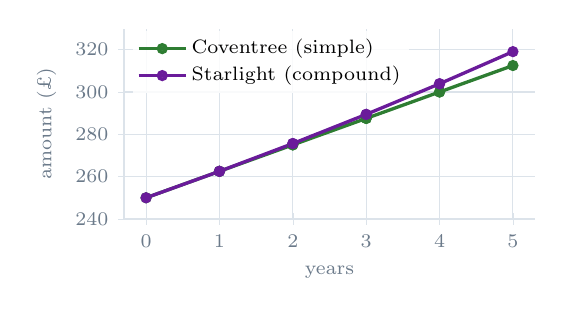
\begin{tikzpicture}
    \begin{axis}[moneyaxis, width=6.8cm, xmin=0,xmax=5,ymin=240,ymax=330,xtick={0,...,5}]
      \legendfor{coventree,very thick,mark=*,mark size=1.4pt}{Coventree (simple)}
      \legendfor{starlight,very thick,mark=*,mark size=1.4pt}{Starlight (compound)}
      \pt{1}{coventree,mark=*,mark size=1.4pt}{(0,250)}
      \seg{1}{coventree,very thick,mark=*,mark size=1.4pt}{(0,250)}{(1,262.5)}
      \seg{2}{coventree,very thick,mark=*,mark size=1.4pt}{(1,262.5)}{(2,275)}
      \seg{3}{coventree,very thick,mark=*,mark size=1.4pt}{(2,275)}{(3,287.5)}
      \seg{4}{coventree,very thick,mark=*,mark size=1.4pt}{(3,287.5)}{(4,300)}
      \seg{5}{coventree,very thick,mark=*,mark size=1.4pt}{(4,300)}{(5,312.5)}
      \seg{1}{starlight,very thick,mark=*,mark size=1.4pt}{(0,250)}{(1,262.5)}
      \seg{2}{starlight,very thick,mark=*,mark size=1.4pt}{(1,262.5)}{(2,275.63)}
      \seg{3}{starlight,very thick,mark=*,mark size=1.4pt}{(2,275.63)}{(3,289.41)}
      \seg{4}{starlight,very thick,mark=*,mark size=1.4pt}{(3,289.41)}{(4,303.88)}
      \seg{5}{starlight,very thick,mark=*,mark size=1.4pt}{(4,303.88)}{(5,319.07)}
    \end{axis}
  \end{tikzpicture}
  \end{plotcard}\\[1mm]
  \uncover<6->{\footnotesize\ealpara{Luka powiększa się co roku.}{The gap gets wider every year.}}
\end{column}
\end{columns}
\end{frame}

% =================================================================
\begin{frame}{Twenty-five years of the same 5\%}
\ealpara{Dwadzieścia pięć lat z tymi samymi 5\%}{Twenty-five years of the same 5\%}
\begin{columns}[T,onlytextwidth]
\begin{column}{0.46\textwidth}
  \begin{card}
    \footnotesize
    \ealpara{\pounds250 na każdym koncie, nadal przy 5\%.}{\pounds250 in each account, still at 5\%.}
    \vspace{1.5mm}
    \begin{tabular}{@{}lrr@{}}
      \toprule
      & Coventree & Starlight\\
      & simple & compound\\
      \midrule
      \rowthree{1}{Year 5}{\pounds312.50}{\pounds319.07}
      \rowthree{2}{Year 10}{\pounds375.00}{\pounds407.22}
      \rowthree{3}{Year 15}{\pounds437.50}{\pounds519.73}
      \rowthree{4}{Year 20}{\pounds500.00}{\pounds663.32}
      \rowthree{5}{Year 25}{\pounds562.50}{\pounds846.59}
      \bottomrule
    \end{tabular}
  \end{card}

  \vspace{1.2mm}
  \uncover<6->{%
  \begin{formulacard}
    \ealpara{Po 25 latach}{After 25 years}
    \vspace{0.6mm}
    \ealpara{prosty: $\pnd 250 (1 + 0.05 \times 25) = \pnd 562.50$}{simple: $\pnd 250 (1 + 0.05 \times 25) = \pnd 562.50$}
    \vspace{0.4mm}
    \ealpara{składany: $\pnd 250 \times 1.05^{25} = \pnd 846.59$}{compound: $\pnd 250 \times 1.05^{25} = \pnd 846.59$}
  \end{formulacard}}
\end{column}
\begin{column}{0.52\textwidth}
  \begin{plotcard}
  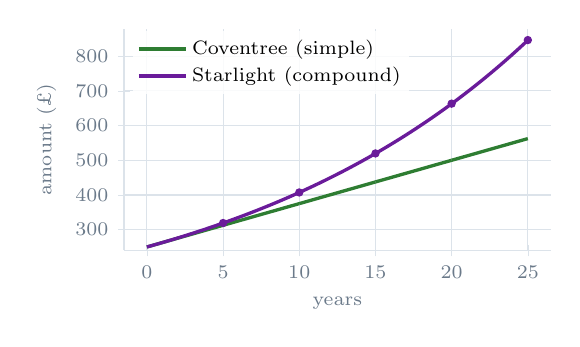
\begin{tikzpicture}
    \begin{axis}[moneyaxis, width=7cm, height=4.4cm,
                 xmin=0,xmax=25,ymin=240,ymax=880,
                 xtick={0,5,10,15,20,25}, ytick={300,400,500,600,700,800}]
      \legendfor{coventree,very thick}{Coventree (simple)}
      \legendfor{starlight,very thick}{Starlight (compound)}
      \curveseg{1}{coventree,very thick}{0}{5}{250*(1+0.05*x)}
      \curveseg{2}{coventree,very thick}{5}{10}{250*(1+0.05*x)}
      \curveseg{3}{coventree,very thick}{10}{15}{250*(1+0.05*x)}
      \curveseg{4}{coventree,very thick}{15}{20}{250*(1+0.05*x)}
      \curveseg{5}{coventree,very thick}{20}{25}{250*(1+0.05*x)}
      \curveseg{1}{starlight,very thick}{0}{5}{250*exp(x*ln(1.05))}
      \curveseg{2}{starlight,very thick}{5}{10}{250*exp(x*ln(1.05))}
      \curveseg{3}{starlight,very thick}{10}{15}{250*exp(x*ln(1.05))}
      \curveseg{4}{starlight,very thick}{15}{20}{250*exp(x*ln(1.05))}
      \curveseg{5}{starlight,very thick}{20}{25}{250*exp(x*ln(1.05))}
      \pt{1}{starlight,mark=*,mark size=1.3pt}{(5,319.07)}
      \pt{2}{starlight,mark=*,mark size=1.3pt}{(10,407.22)}
      \pt{3}{starlight,mark=*,mark size=1.3pt}{(15,519.73)}
      \pt{4}{starlight,mark=*,mark size=1.3pt}{(20,663.32)}
      \pt{5}{starlight,mark=*,mark size=1.3pt}{(25,846.59)}
    \end{axis}
  \end{tikzpicture}
  \end{plotcard}\\[1mm]
  \uncover<6->{\footnotesize\ealpara{Linia \ealkeytr{procentu prostego} zachowuje ten sam \ealkeytr{współczynnik kierunkowy}, podczas gdy \ealkeytr{krzywa} \ealkeytr{procentu składanego} staje się coraz bardziej stroma. Po 25 latach \ealkeytr{różnica} wynosi \pounds284.09.}{The simple \ealkey{interest} line keeps the same \ealkey{gradient}, while the compound \ealkey{curve} gets steeper every year. After 25 years the \ealkey{difference} is \pounds284.09.}}
\end{column}
\end{columns}
\end{frame}

% =================================================================
\begin{frame}{\bank{virgo}{Virgo Money} 8\% compound over thirty years}
\ealpara{\bank{virgo}{Virgo Money} 8\% składany przez trzydzieści lat}{\bank{virgo}{Virgo Money} 8\% compound over thirty years}
\begin{columns}[T,onlytextwidth]
\begin{column}{0.48\textwidth}
  \begin{card}[virgo]
    \footnotesize
    \ealpara{Dev wpłaca \pounds1000 i zostawia to. Druga kolumna to te same \pounds1000 przy 8\% \emph{procencie prostym}.}{Dev pays in \pounds1000 and leaves it alone. The second column is the same \pounds1000 at 8\% \emph{simple interest}.}
    \vspace{1.5mm}
    \begin{tabular}{@{}lrr@{}}
      \toprule
      & simple & compound\\
      \midrule
      \rowthree{1}{Year 10}{\pounds1800}{\pounds2158.92}
      \rowthree{2}{Year 20}{\pounds2600}{\pounds4660.96}
      \rowthree{3}{Year 30}{\pounds3400}{\pounds10062.66}
      \bottomrule
    \end{tabular}
  \end{card}

  \vspace{1.2mm}
  \uncover<4->{%
  \begin{formulacard}[virgo]
    \ealpara{Po 30 latach}{After 30 years}
    \vspace{0.6mm}
    \ealpara{prosty: $\pnd 1000 (1 + 0.08 \times 30) = \pnd 3400$}{simple: $\pnd 1000 (1 + 0.08 \times 30) = \pnd 3400$}
    \vspace{0.4mm}
    \ealpara{składany: $\pnd 1000 \times 1.08^{30} = \pnd 10062.66$}{compound: $\pnd 1000 \times 1.08^{30} = \pnd 10062.66$}
  \end{formulacard}}
\end{column}
\begin{column}{0.50\textwidth}
  \begin{plotcard}[virgo]
  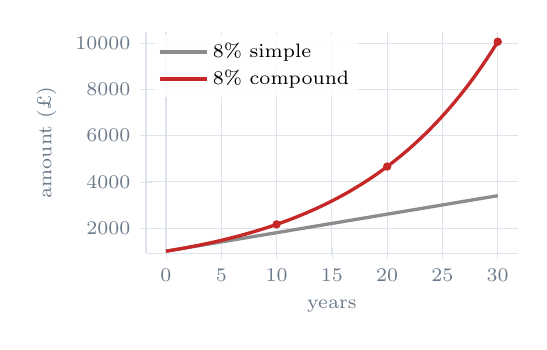
\begin{tikzpicture}
    \begin{axis}[moneyaxis, width=6.3cm, height=4.4cm,
                 xmin=0,xmax=30,ymin=900,ymax=10500,
                 xtick={0,5,10,15,20,25,30},
                 ytick={2000,4000,6000,8000,10000}]
      \legendfor{black!45,very thick}{8\% simple}
      \legendfor{virgo,very thick}{8\% compound}
      \curveseg{1}{black!45,very thick}{0}{10}{1000*(1+0.08*x)}
      \curveseg{2}{black!45,very thick}{10}{20}{1000*(1+0.08*x)}
      \curveseg{3}{black!45,very thick}{20}{30}{1000*(1+0.08*x)}
      \curveseg{1}{virgo,very thick}{0}{10}{1000*exp(x*ln(1.08))}
      \curveseg{2}{virgo,very thick}{10}{20}{1000*exp(x*ln(1.08))}
      \curveseg{3}{virgo,very thick}{20}{30}{1000*exp(x*ln(1.08))}
      \pt{1}{virgo,mark=*,mark size=1.3pt}{(10,2158.92)}
      \pt{2}{virgo,mark=*,mark size=1.3pt}{(20,4660.96)}
      \pt{3}{virgo,mark=*,mark size=1.3pt}{(30,10062.66)}
    \end{axis}
  \end{tikzpicture}
  \end{plotcard}\\[1mm]
  \uncover<4->{\footnotesize\ealpara{\ealkeytr{Suma} składana w przybliżeniu \ealkeytr{podwaja się} co 9 lat: około \pounds2000 po 9 latach, \pounds4000 po 18 latach i \pounds8000 po 27 latach.}{The compound \ealkey{total} \ealkey{doubles} roughly every 9 years: about \pounds2000 at 9 years, \pounds4000 at 18 years and \pounds8000 at 27 years.}}
\end{column}
\end{columns}
\end{frame}

% =================================================================
\newcommand{\priyaQuestions}[1]{%
  \ealpara{Przez co mnożymy co roku?}{What do we multiply by each year? \hfill #1{1.06}}\vspace{\qgap}
  \ealpara{Ile po 10 latach?}{How much after 10 years? \hfill #1{\pounds895.42}}\vspace{\qgap}
  \ealpara{Po ilu pełnych latach jest więcej niż \pounds1000?}{After how many whole years is there more than \pounds1000? \hfill #1{12 years}}}

\begin{frame}{\wb\ \ How long does the money take to \ealkey{double}?}
\ealpara{\wb\ \ Jak długo trwa, zanim pieniądze się \ealkeytr{podwoją}?}{\wb\ \ How long does the money take to \ealkey{double}?}
\begin{questionblock}
  \ealpara{\bank{starlight}{Starlight Bank} oferuje również 6\% \ealkeytr{procentu składanego} rocznie.}{\normalsize\raggedright\bank{starlight}{Starlight Bank} also offers 6\% \ealkey{compound interest} per year.\par}
  \vspace{3mm}

  \ealpara{Priya wpłaca \pounds500 i zostawia je tam.}{\textbf{Priya pays in \pounds500 and leaves it there.}}
  \vspace{7mm}
  \priyaQuestions{\ablank}
\end{questionblock}
\end{frame}

\begin{frame}{\sol\ \ How long does the money take to \ealkey{double}?}
\ealpara{\sol\ \ Jak długo trwa, zanim pieniądze się \ealkeytr{podwoją}?}{\sol\ \ How long does the money take to \ealkey{double}?}
\ealpara{\bank{starlight}{Starlight Bank} 6\% \ealkeytr{procentu składanego} rocznie.}{\bank{starlight}{Starlight Bank} 6\% \ealkey{compound interest} per year.}
\ealpara{Priya wpłaca \pounds500.}{\textbf{Priya pays in \pounds500.}}
\vspace{2mm}

\begin{columns}[T,onlytextwidth]
\begin{column}{0.52\textwidth}
  \priyaQuestions{\ashow}

  \vspace{3mm}
  \uncover<4->{%
  {\footnotesize\ealpara{Przy 6\% \emph{procencie prostym} te same \pounds500 nie przekracza \pounds1000 aż do roku 17, ponieważ $\pnd 500 (1 + 0.06 \times 17) = \pnd 1010$.}{At 6\% \emph{simple interest} the same \pounds500 does not pass \pounds1000 until year 17, because $\pnd 500 (1 + 0.06 \times 17) = \pnd 1010$.}}}
\end{column}
\begin{column}{0.44\textwidth}
  \begin{card}[starlight]
    \footnotesize
    \begin{tabular}{@{}lr@{}}
      \toprule
      & \ealkey{total}\\
      \midrule
      \rowtwo{1}{Year 10}{\pounds895.42}
      \rowtwo{2}{Year 11}{\pounds949.15}
      \rowtwo{3}{Year 12}{\pounds1006.10}
      \bottomrule
    \end{tabular}
  \end{card}

  \vspace{1.2mm}
  \uncover<4->{%
  \begin{formulacard}[starlight]
    $\pnd 500 \times 1.06^{12} = \pnd 1006.10$\\[0.6mm]
    \ashow{\ealpara{\ealkeytr{Procent składany} \ealkeytr{podwaja} pieniądze w 12 lat, \ealkeytr{procent prosty} w 17.}{\ealkey{Compound interest} \ealkey{doubles} the money in 12 years, \ealkey{simple interest} in 17.}}
  \end{formulacard}}
\end{column}
\end{columns}
\end{frame}

% =================================================================
\begin{frame}{\bank{tesbury}{Tesbury Bank} 6\% simple --- but \ealkey{locked in} for 2 years}
\ealpara{\bank{tesbury}{Tesbury Bank} 6\% prosty --- ale \ealkeytr{zablokowane} na 2 lata}{\bank{tesbury}{Tesbury Bank} 6\% simple --- but \ealkey{locked in} for 2 years}
\ealpara{Chloe wpłaca \pounds400 i zostawia je na 4 lata.}{\textbf{Chloe puts in \pounds400 and leaves it for 4 years.}}
\vspace{1.5mm}

\begin{columns}[T,onlytextwidth]
\begin{column}{0.42\textwidth}
  \begin{card}[tesbury]
    \footnotesize
    \ealpara{6\% z \pounds400 to \pounds24 co roku.}{6\% of \pounds400 is \pounds24 every year.}
    \vspace{1.5mm}
    \begin{tabular}{@{}lrr@{}}
      \toprule
      & \ealkey{interest} & \ealkey{total}\\
      \midrule
      \rowthree{1}{Start}{}{\pounds400}
      \rowthree{2}{Year 1}{\pounds24}{\pounds424}
      \rowthree{3}{Year 2}{\pounds24}{\pounds448}
      \rowthree{4}{Year 3}{\pounds24}{\pounds472}
      \rowthree{5}{Year 4}{\pounds24}{\pounds496}
      \bottomrule
    \end{tabular}
  \end{card}

  \vspace{1.2mm}
  \uncover<6->{%
  \begin{formulacard}[tesbury]
    \ealpara{Stosując \ealkeytr{wzór}}{Using the \ealkey{formula}}
    \vspace{0.6mm}
    \ealpara{\ealkeytr{suma} $= P(1+rn)$}{\ealkey{total} $= P(1+rn)$}
    \vspace{0.4mm}
    \hspace*{3mm}$= \pnd 400 (1 + 0.06 \times 4) = \pnd 496$
  \end{formulacard}}
\end{column}
\begin{column}{0.56\textwidth}
  \begin{plotcard}[tesbury]
  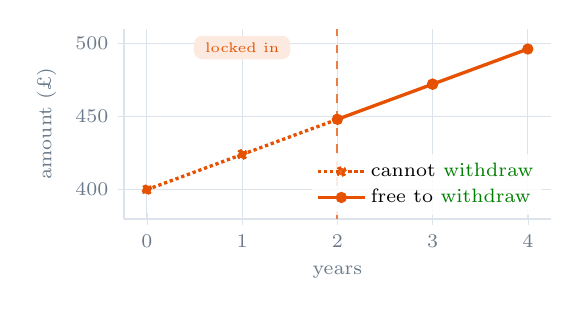
\begin{tikzpicture}
    \begin{axis}[moneyaxis, width=7cm, xmin=0,xmax=4,ymin=380,ymax=510,xtick={0,...,4},
                 legend style={at={(0.98,0.02)},anchor=south east}]
      \draw[tesbury!75,dashed,thick] (axis cs:2,380) -- (axis cs:2,510);
      \lockedlabel{tesbury}{1}{497}
      \legendfor{tesbury,very thick,densely dotted,mark=*,mark size=1.4pt}
                {cannot \ealkey{withdraw}}
      \legendfor{tesbury,very thick,mark=*,mark size=1.4pt}{free to \ealkey{withdraw}}
      \pt{1}{tesbury,mark=*,mark size=1.4pt}{(0,400)}
      \seg{2}{tesbury,very thick,densely dotted,mark=*,mark size=1.4pt}{(0,400)}{(1,424)}
      \seg{3}{tesbury,very thick,densely dotted,mark=*,mark size=1.4pt}{(1,424)}{(2,448)}
      \seg{4}{tesbury,very thick,mark=*,mark size=1.4pt}{(2,448)}{(3,472)}
      \seg{5}{tesbury,very thick,mark=*,mark size=1.4pt}{(3,472)}{(4,496)}
    \end{axis}
  \end{tikzpicture}
  \end{plotcard}\\[1mm]
  \uncover<6->{\footnotesize\ealpara{\textbf{Kropkowana} część to czas, gdy pieniądze są \ealkeytr{zablokowane}.}{The \textbf{dotted} part is while the money is \ealkey{locked in}.}}
\end{column}
\end{columns}
\end{frame}

% =================================================================
\newcommand{\erinOffers}{%
  \ealpara{\bank{virgo}{Virgo Money} 8\% \textbf{składany} rocznie}{\bank{virgo}{Virgo Money} 8\% \textbf{compound} per year}\vspace{4mm}
  \ealpara{\bank{tesbury}{Tesbury Bank} 6\% \textbf{prosty} rocznie}{\bank{tesbury}{Tesbury Bank} 6\% \textbf{simple} per year}}

\begin{frame}{\wb\ \ Which account, and by how much?}
\ealpara{\wb\ \ Które konto i o ile?}{\wb\ \ Which account, and by how much?}
\begin{questionblock}
  \ealpara{Erin ma \pounds600 do oszczędzania na 2 lata.}{\textbf{Erin has \pounds600 to save for 2 years.}}
  \vspace{7mm}
  \erinOffers
  \vspace{7mm}
  \ealpara{Które daje jej więcej i jaka jest \ealkeytr{różnica}?}{Which gives her more, and what is the \ealkey{difference}?}
\end{questionblock}
\end{frame}

\begin{frame}{\sol\ \ Which account, and by how much?}
\ealpara{\sol\ \ Które konto i o ile?}{\sol\ \ Which account, and by how much?}
\ealpara{Erin ma \pounds600 do oszczędzania na 2 lata.}{\textbf{Erin has \pounds600 to save for 2 years.}}
\vspace{2mm}

\begin{columns}[T,onlytextwidth]
\begin{column}{0.5\textwidth}
  \erinOffers
  \vspace{5mm}
  \uncover<3->{\ashow{\ealpara{Virgo płaci jej o \pounds27.84 więcej.}{Virgo pays her \pounds27.84 more.}}}

  \vspace{3mm}
  \uncover<4->{%
  \begin{formulacard}
    \ealpara{Stosując \ealkeytr{wzory}}{Using the \ealkey{formulas}}
    \vspace{0.6mm}
    \ealpara{Virgo: $\pnd 600 \times 1.08^{2} = \pnd 699.84$}{Virgo: $\pnd 600 \times 1.08^{2} = \pnd 699.84$}
    \vspace{0.4mm}
    \ealpara{Tesbury: $\pnd 600 (1 + 0.06 \times 2) = \pnd 672$}{Tesbury: $\pnd 600 (1 + 0.06 \times 2) = \pnd 672$}
  \end{formulacard}}
\end{column}
\begin{column}{0.46\textwidth}
  \begin{card}
    \footnotesize
    \begin{tabular}{@{}lrr@{}}
      \toprule
      & Virgo & Tesbury\\
      \midrule
      \rowthree{1}{Start}{\pounds600.00}{\pounds600}
      \rowthree{2}{Year 1}{\pounds648.00}{\pounds636}
      \rowthree{3}{Year 2}{\pounds699.84}{\pounds672}
      \bottomrule
    \end{tabular}
  \end{card}
\end{column}
\end{columns}
\end{frame}

% =================================================================
\begin{frame}{\bank{santandra}{Santandra} 8\% compound --- \ealkey{locked in} for 2 years}
\ealpara{\bank{santandra}{Santandra} 8\% składany --- \ealkeytr{zablokowane} na 2 lata}{\bank{santandra}{Santandra} 8\% compound --- \ealkey{locked in} for 2 years}
\ealpara{Dev wpłaca \pounds1000 i zostawia je na 3 lata.}{\textbf{Dev puts in \pounds1000 and leaves it for 3 years.}}
\vspace{1.5mm}

\begin{columns}[T,onlytextwidth]
\begin{column}{0.42\textwidth}
  \begin{card}[santandra]
    \footnotesize
    \ealpara{\ealkeytr{Mnożnik} wynosi $1.08$, raz na każdy rok.}{The \ealkey{multiplier} is $1.08$, once for each year.}
    \vspace{1.5mm}
    \begin{tabular}{@{}lrr@{}}
      \toprule
      & \ealkey{interest} & \ealkey{total}\\
      \midrule
      \rowthree{1}{Start}{}{\pounds1000.00}
      \rowthree{2}{Year 1}{\pounds80.00}{\pounds1080.00}
      \rowthree{3}{Year 2}{\pounds86.40}{\pounds1166.40}
      \rowthree{4}{Year 3}{\pounds93.31}{\pounds1259.71}
      \bottomrule
    \end{tabular}
  \end{card}

  \vspace{1.2mm}
  \uncover<5->{%
  \begin{formulacard}[santandra]
    \ealpara{Stosując \ealkeytr{wzór}}{Using the \ealkey{formula}}
    \vspace{0.6mm}
    \ealpara{\ealkeytr{suma} $= P(1+r)^{n}$}{\ealkey{total} $= P(1+r)^{n}$}
    \vspace{0.4mm}
    \hspace*{3mm}$= \pnd 1000 \times 1.08^{3} = \pnd 1259.71$
  \end{formulacard}}
\end{column}
\begin{column}{0.56\textwidth}
  \begin{plotcard}[santandra]
  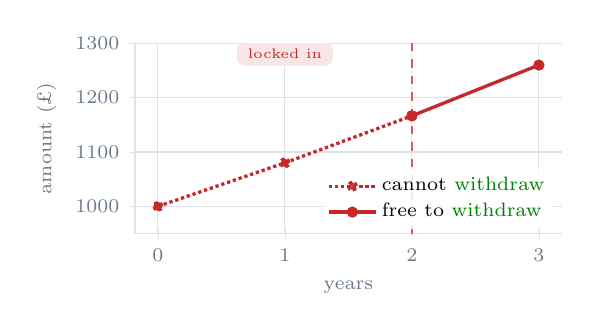
\begin{tikzpicture}
    \begin{axis}[moneyaxis, width=7cm, xmin=0,xmax=3,ymin=950,ymax=1300,xtick={0,1,2,3},
                 legend style={at={(0.98,0.02)},anchor=south east}]
      \draw[santandra!75,dashed,thick] (axis cs:2,950) -- (axis cs:2,1300);
      \lockedlabel{santandra}{1}{1280}
      \legendfor{santandra,very thick,densely dotted,mark=*,mark size=1.4pt}
                {cannot \ealkey{withdraw}}
      \legendfor{santandra,very thick,mark=*,mark size=1.4pt}{free to \ealkey{withdraw}}
      \pt{1}{santandra,mark=*,mark size=1.4pt}{(0,1000)}
      \seg{2}{santandra,very thick,densely dotted,mark=*,mark size=1.4pt}{(0,1000)}{(1,1080)}
      \seg{3}{santandra,very thick,densely dotted,mark=*,mark size=1.4pt}{(1,1080)}{(2,1166.4)}
      \seg{4}{santandra,very thick,mark=*,mark size=1.4pt}{(2,1166.4)}{(3,1259.71)}
    \end{axis}
  \end{tikzpicture}
  \end{plotcard}\\[1mm]
  \uncover<5->{\footnotesize\ealpara{Pieniądze Dev'a są \ealkeytr{zablokowane} przez pierwsze 2 lata, więc to konto nie jest dla niego przydatne, jeśli potrzebuje gotówki wcześniej.}{Dev's money is \ealkey{locked in} for the first 2 years, so this account is no use to him if he needs the cash sooner.}}
\end{column}
\end{columns}
\end{frame}

% =================================================================
\begin{frame}{Read the small print}
\ealpara{Przeczytaj drobny druk}{Read the small print}
\ealpara{\bank{metroline}{Metroline Bank} płaci 10\%, najwyższą \ealkeytr{wielkość ilorazową} na arkuszu, ale przyjmuje \pounds300 \ealkeytr{maksimum}.}{\bank{metroline}{Metroline Bank} pays 10\%, the highest \ealkey{rate} on the sheet, but takes \pounds300 \ealkey{maximum}.}
\ealpara{Dev ma \pounds1000 do oszczędzania na 3 lata.}{\textbf{Dev has \pounds1000 to save for 3 years.}}
\vspace{1.5mm}

\begin{columns}[T,onlytextwidth]
\begin{column}{0.46\textwidth}
  \begin{card}[metroline]
    \footnotesize
    \ealpara{Tylko \pounds300 jest dozwolone na koncie.}{Only \pounds300 is allowed in the account.}
    \vspace{1.5mm}
    \begin{tabular}{@{}lrr@{}}
      \toprule
      after 3 years & in account & \ealkey{total}\\
      \midrule
      \rowthree{5}{Metroline}{\pounds390.00}{\pounds1090.00}
      \rowthree{5}{Virgo (8\%)}{\pounds1259.71}{\pounds1259.71}
      \bottomrule
    \end{tabular}
  \end{card}

  \vspace{1.2mm}
  \uncover<5->{%
  \begin{formulacard}[metroline]
    \ealpara{Stosując \ealkeytr{wzory}}{Using the \ealkey{formulas}}
    \vspace{0.6mm}
    \ealpara{Metroline: $\pnd 300 (1 + 0.10 \times 3) = \pnd 390$,}{Metroline: $\pnd 300 (1 + 0.10 \times 3) = \pnd 390$,}
    \vspace{0.4mm}
    \ealpara{a \pounds700 pozostawione w domu daje \pounds1090}{and the \pounds700 left at home makes \pounds1090}
    \vspace{0.4mm}
    \ealpara{Virgo: $\pnd 1000 \times 1.08^{3} = \pnd 1259.71$}{Virgo: $\pnd 1000 \times 1.08^{3} = \pnd 1259.71$}
  \end{formulacard}}
\end{column}
\begin{column}{0.52\textwidth}
  \begin{plotcard}[metroline]
  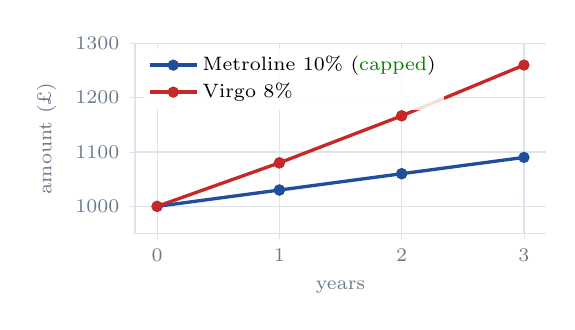
\begin{tikzpicture}
    \begin{axis}[moneyaxis, width=6.8cm, xmin=0,xmax=3,ymin=950,ymax=1300,xtick={0,1,2,3},
                 legend style={at={(0.02,0.98)}}]
      \legendfor{metroline,very thick,mark=*,mark size=1.4pt}{Metroline 10\% (\ealkey{capped})}
      \legendfor{virgo,very thick,mark=*,mark size=1.4pt}{Virgo 8\%}
      \pt{1}{metroline,mark=*,mark size=1.4pt}{(0,1000)}
      \seg{2}{metroline,very thick,mark=*,mark size=1.4pt}{(0,1000)}{(1,1030)}
      \seg{3}{metroline,very thick,mark=*,mark size=1.4pt}{(1,1030)}{(2,1060)}
      \seg{4}{metroline,very thick,mark=*,mark size=1.4pt}{(2,1060)}{(3,1090)}
      \seg{2}{virgo,very thick,mark=*,mark size=1.4pt}{(0,1000)}{(1,1080)}
      \seg{3}{virgo,very thick,mark=*,mark size=1.4pt}{(1,1080)}{(2,1166.4)}
      \seg{4}{virgo,very thick,mark=*,mark size=1.4pt}{(2,1166.4)}{(3,1259.71)}
    \end{axis}
  \end{tikzpicture}
  \end{plotcard}\\[1mm]
  \uncover<5->{\footnotesize\ealpara{Największy \ealkeytr{procent} nie zawsze jest najlepszą ofertą.}{The biggest \ealkey{percentage} is not always the best deal.}}
\end{column}
\end{columns}
\end{frame}

% =================================================================
\newcommand{\aishaQuestions}[1]{%
  \ealpara{Ile po 6 miesiącach?}{How much after 6 months? \hfill #1{\pounds510}}\vspace{\qgap}
  \ealpara{Ile po 12 miesiącach?}{How much after 12 months? \hfill #1{\pounds520.20}}\vspace{\qgap}
  \ealpara{Czy 2\% dwa razy w roku to to samo co 4\% raz w roku?}{Is 2\% twice a year the same as 4\% once a year?}}

\begin{frame}{\wb\ \ Interest paid twice a year}
\ealpara{\wb\ \ \ealkeytr{Odsetki} wypłacane dwa razy w roku}{\wb\ \ \ealkey{Interest} paid twice a year}
\begin{questionblock}
  \ealpara{\bank{halifield}{Halifield} Half-Year Saver: 2\% \ealkeytr{procent składany} co sześć miesięcy.}{\normalsize\raggedright\bank{halifield}{Halifield} Half-Year Saver: 2\% \ealkey{compound interest} every six months.\par}
  \vspace{3mm}

  \ealpara{Aisha wpłaca \pounds500 na jeden rok.}{\textbf{Aisha puts in \pounds500 for one year.}}
  \vspace{7mm}
  \aishaQuestions{\ablank}
\end{questionblock}
\end{frame}

\begin{frame}{\sol\ \ Interest paid twice a year}
\ealpara{\sol\ \ \ealkeytr{Odsetki} wypłacane dwa razy w roku}{\sol\ \ \ealkey{Interest} paid twice a year}
\ealpara{\bank{halifield}{Halifield} Half-Year Saver: 2\% \ealkeytr{procent składany} co sześć miesięcy.}{\bank{halifield}{Halifield} Half-Year Saver: 2\% \ealkey{compound interest} every six months.}
\ealpara{Aisha wpłaca \pounds500 na jeden rok.}{\textbf{Aisha puts in \pounds500 for one year.}}
\vspace{2mm}

\begin{columns}[T,onlytextwidth]
\begin{column}{0.5\textwidth}
  \aishaQuestions{\ashow}\\[1mm]
  \uncover<3->{\ashow{\ealpara{Nie --- \pounds520.20 w porównaniu z \pounds520.}{No --- \pounds520.20 against \pounds520.}}}

  \vspace{1.6mm}
  \uncover<4->{%
  \begin{formulacard}[halifield]
    \ealpara{Stosując \ealkeytr{wzór}}{Using the \ealkey{formula}}
    \vspace{0.6mm}
    \ealpara{Tutaj $n = 2$, ponieważ \ealkeytr{odsetki} są dodawane dwa razy:}{Here $n = 2$, because the \ealkey{interest} is added twice:}
    \vspace{0.4mm}
    \ealpara{\ealkeytr{suma} $= \pnd 500 \times 1.02^{2} = \pnd 520.20$}{\ealkey{total} $= \pnd 500 \times 1.02^{2} = \pnd 520.20$}
  \end{formulacard}}
\end{column}
\begin{column}{0.46\textwidth}
  \begin{card}[halifield]
    \footnotesize
    \begin{tabular}{@{}lrr@{}}
      \toprule
      & \ealkey{interest} & \ealkey{total}\\
      \midrule
      \rowthree{1}{Start}{}{\pounds500.00}
      \rowthree{2}{6 months}{\pounds10.00}{\pounds510.00}
      \rowthree{3}{12 months}{\pounds10.20}{\pounds520.20}
      \bottomrule
    \end{tabular}\\[2mm]
    \uncover<4->{\ealpara{$1.02 \times 1.02 = 1.0404$, więc to wychodzi jako 4.04\% za rok.}{$1.02 \times 1.02 = 1.0404$, so it works out as 4.04\% for the year.}}
  \end{card}
\end{column}
\end{columns}
\end{frame}

% =================================================================
\newcommand{\sofiaQuestions}[1]{%
  \ealpara{Ile \ealkeytr{odsetek} w 2 lata?}{How much \ealkey{interest} in 2 years? \hfill #1{\pounds30}}\vspace{\qgap}
  \ealpara{Ile kosztują \ealkeytr{opłaty}?}{How much do the \ealkey{fees} cost? \hfill #1{\pounds48}}\vspace{\qgap}
  \ealpara{Z czym zostaje?}{What is she left with? \hfill #1{\pounds232}}}

\begin{frame}{\wb\ \ Challenge: a \pounds2 monthly \ealkey{fee}}
\ealpara{\wb\ \ Wyzwanie: miesięczna \ealkeytr{opłata} \pounds2}{\wb\ \ Challenge: a \pounds2 monthly \ealkey{fee}}
\begin{questionblock}
  \ealpara{\bank{nationworth}{Nationworth} Loyalty Saver: 6\% \ealkeytr{procent prosty}, \pounds2 \ealkeytr{opłata} co miesiąc.}{\normalsize\raggedright\bank{nationworth}{Nationworth} Loyalty Saver: 6\% \ealkey{simple interest}, \pounds2 \ealkey{fee} every month.\par}
  \vspace{3mm}

  \ealpara{Sofia wpłaca \pounds250 na 2 lata.}{\textbf{Sofia puts in \pounds250 for 2 years.}}
  \vspace{7mm}
  \sofiaQuestions{\ablank}
\end{questionblock}
\end{frame}

\begin{frame}{\sol\ \ Challenge: a \pounds2 monthly \ealkey{fee}}
\ealpara{\sol\ \ Wyzwanie: miesięczna \ealkeytr{opłata} \pounds2}{\sol\ \ Challenge: a \pounds2 monthly \ealkey{fee}}
\ealpara{\bank{nationworth}{Nationworth} Loyalty Saver: 6\% \ealkeytr{procent prosty}, \pounds2 \ealkeytr{opłata} co miesiąc.}{\bank{nationworth}{Nationworth} Loyalty Saver: 6\% \ealkey{simple interest}, \pounds2 \ealkey{fee} every month.}
\ealpara{Sofia wpłaca \pounds250 na 2 lata.}{\textbf{Sofia puts in \pounds250 for 2 years.}}
\vspace{2mm}

\begin{columns}[T,onlytextwidth]
\begin{column}{0.5\textwidth}
  \sofiaQuestions{\ashow}

  \vspace{3.4mm}
  \uncover<5->{%
  \begin{formulacard}[nationworth]
    \ealpara{Stosując \ealkeytr{wzór}}{Using the \ealkey{formula}}
    \vspace{0.6mm}
    \ealpara{\ealkeytr{odsetki} $= P \times r \times n$}{\ealkey{interest} $= P \times r \times n$}
    \vspace{0.4mm}
    \hspace*{3mm}$= \pnd 250 \times 0.06 \times 2 = \pnd 30$
    \vspace{0.4mm}
    \ealpara{Ile musiałaby wpłacić, zanim to konto przestanie tracić jej pieniądze?}{How much would she need to pay in before this account stops losing her money?}
  \end{formulacard}}
\end{column}
\begin{column}{0.46\textwidth}
  \begin{card}[nationworth]
    \footnotesize
    \begin{tabular}{@{}lr@{}}
      \toprule
      \rowtwo{1}{Paid in}{\pounds250}
      \rowtwo{2}{\ealkey{Interest} (2 years)}{$+$ \pounds30}
      \rowtwo{3}{\ealkey{Fees} ($24 \times 2$)}{$-$ \pounds48}
      \midrule
      \rowtwo{4}{\textbf{\ealkey{Total}}}{\textbf{\pounds232}}
      \bottomrule
    \end{tabular}\\[2mm]
    \uncover<4->{\ashow{\ealpara{Kończy z mniejszą kwotą, niż zaczęła.}{She ends up with less than she started with.}}}
  \end{card}
\end{column}
\end{columns}
\end{frame}

% =================================================================
\begin{frame}{Choosing an account}
\ealpara{Wybór konta}{Choosing an account}
\begin{columns}[T,onlytextwidth]
\begin{column}{0.56\textwidth}
  \begin{card}[slidehead]
    \small
    \begin{itemize}[<+->]\itemsep=1.4mm
      \item \ealpara{\textbf{Procent prosty} to ta sama kwota co roku. \textbf{Procent składany} rośnie.}{\textbf{\ealkey{Simple interest}} is the same amount every year. \textbf{\ealkey{Compound interest}} grows.}
      \item \ealpara{Przy tej samej \ealkeytr{wielkości ilorazowej}, \ealkeytr{procent składany} zawsze płaci co najmniej tyle samo, a luka rośnie im dłużej pieniądze są zostawione.}{At the same \ealkey{rate}, \ealkey{compound interest} always pays at least as much, and the gap grows the longer the money is left.}
      \item \ealpara{Duży \ealkeytr{procent} na nic się nie zda, jeśli istnieje \ealkeytr{maksimum}, które możesz wpłacić.}{A big \ealkey{percentage} is no use if there is a \ealkey{maximum} you can pay in.}
      \item \ealpara{Konto \ealkeytr{zablokowane} na nic się nie zda, jeśli potrzebujesz pieniędzy wcześniej.}{A \textbf{locked} account is no use if you need the money sooner.}
      \item \ealpara{\ealkeytr{Opłata} może całkowicie pochłonąć \ealkeytr{odsetki}.}{A \ealkey{fee} can swallow the \ealkey{interest} completely.}
    \end{itemize}
  \end{card}
\end{column}
\begin{column}{0.42\textwidth}
  \begin{formulacard}[slidehead]
    \ealpara{Te dwa \ealkeytr{wzory}}{The two \ealkey{formulas}}
    \vspace{1.5mm}
    \ealpara{procent prosty: \ealkeytr{suma} $= P(1+rn)$}{simple: \ealkey{total} $= P(1+rn)$}
    \vspace{1mm}
    \ealpara{procent składany: \ealkeytr{suma} $= P(1+r)^{n}$}{compound: \ealkey{total} $= P(1+r)^{n}$}
    \vspace{1.5mm}
    \ealpara{$P$ to kwota wpłacona, $r$ to \ealkeytr{wielkość ilorazowa} \ealkeytr{odsetek} zapisana jako \ealkeytr{ułamek dziesiętny}, a $n$ to liczba lat.}{$P$ is the amount paid in, $r$ is the \ealkey{interest} \ealkey{rate} written as a \ealkey{decimal} and $n$ is the number of years.}
  \end{formulacard}

  \vspace{2mm}
  \uncover<5->{%
  \begin{card}[slidehead]
    \centering\small
    \ealpara{\textbf{Oblicz \ealkeytr{sumę}, potem sprawdź drobny druk.}}{\textbf{Work out the \ealkey{total}, then check the small print.}}
  \end{card}}
\end{column}
\end{columns}
\end{frame}

\end{document}